\documentclass[aspectratio=169]{beamer}

\usepackage{amsmath}
\usepackage{booktabs}
\usepackage{xcolor}
\usepackage[english]{babel}
%\usepackage{unicode-math}
\usepackage{mathtools}
%\usepackage{derivative}
%\usepackage{makecell}
%\usepackage{multirow}
\usepackage{siunitx}
%\usepackage{pgfplots}
\usepackage{circuitikz}
%\usepackage{appendixnumberbeamer}

\usetheme{metropolis}

%\setmainfont{Stix Two Text}
%\setmathfont{Stix Two Math}

%\pgfplotsset{compat=1.17}
\renewcommand{\familydefault}{\sfdefault}
\usetikzlibrary{arrows.meta}
\usetikzlibrary{fit}
\usetikzlibrary{positioning}
%\usetikzlibrary{shapes.geometric}
%\usetikzlibrary{shapes.misc}
%\usepgfplotslibrary{groupplots}

\DeclarePairedDelimiter{\ceil}{\lceil}{\rceil}
\DeclarePairedDelimiter{\floor}{\lfloor}{\rfloor}
\DeclarePairedDelimiter{\abs}{\lvert}{\rvert}
\DeclarePairedDelimiter{\norm}{\lVert}{\rVert}
\DeclarePairedDelimiter{\bra}{\langle}{\rvert}
\DeclarePairedDelimiter{\ket}{\lvert}{\rangle}
\DeclarePairedDelimiter{\expval}{\langle}{\rangle}
\DeclarePairedDelimiter{\norder}{\mathcolon}{\mathcolon}
\DeclarePairedDelimiter{\anorder}{\typecolon}{\typecolon}
	
\newcommand{\laplace}{\mbfnabla^2}
\newcommand{\trans}{{\scriptscriptstyle\mathsf{T}}}

\newcommand{\conv}{\ast}
\newcommand{\vdot}{\cdot}
\newcommand{\vcross}{\vectimes}
\newcommand{\vb}[1]{\symbfup{#1}}
\newcommand{\vu}[1]{\hat{\vb{#1}}}
\newcommand*\dd[2][\relax]{\mathop{\ifx\relax#1\odif{#2}\else \odif[order={#1}]{#2}\fi}}

\newcommand{\vacket}{\ket*{0}}
\newcommand{\vacbra}{\bra*{0}}

\DeclareMathOperator{\trace}{Tr}
\DeclareMathOperator{\sinc}{sinc}

\AtBeginDocument{
	\let\Re\relax
	\let\Im\relax
	\DeclareMathOperator{\Re}{Re}
	\DeclareMathOperator{\Im}{Im}

	\renewcommand{\div}{\mathop{\mbfnabla\vdot}}
	\newcommand{\curl}{\mathop{\mbfnabla\vectimes}}
}

\DeclarePairedDelimiterX{\comm}[2]{[}{]}{#1,#2}

\DeclarePairedDelimiterX{\braket}[2]{\langle}{\rangle}{#1\delimsize\vert#2}
\DeclarePairedDelimiterX{\ketbra}[1]{\lvert}{\rvert}{#1\rangle\delimsize\langle#1}


\date{\today}
\author{Bodo Kaiser}
\institute{Ryd-Yb Lab}

\begin{document}
	\title{399 nm (blue) laser setup}

	\maketitle
	
	\begin{frame}{Introduction}
		\begin{columns}[T,onlytextwidth]
		    \column{0.6\textwidth}
			\begin{figure}
				\centering
				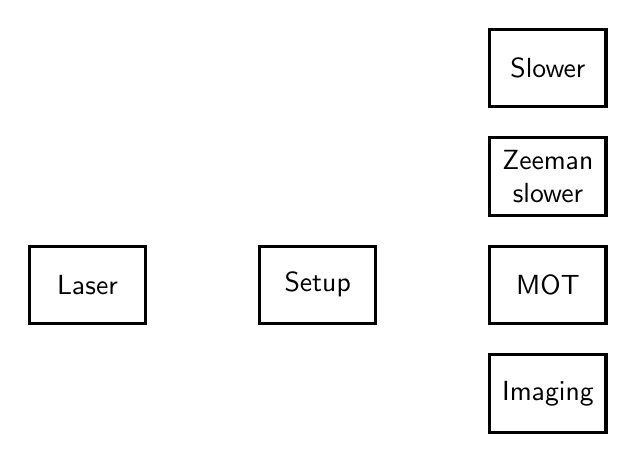
\begin{tikzpicture}[
					node distance=40pt,
					block/.style={draw, very thick, align=center, minimum height=28pt, minimum width=42pt}
				]
					\node[block] (laser) {Laser};
					\node[block, right=of laser] (setup) {Setup};
					\node[block, right=of setup] (mot) {MOT};
					\node[block, above=10pt of mot] (zl) {Zeeman\\slower};
					\node[block, above=10pt of zl] (sl) {Slower};
					\node[block, below=10pt of mot] (imag) {Imaging};
				\end{tikzpicture}
				\caption{Block diagram of the \SI{399}{\nano\meter} setup.}
			\end{figure}

		    \column{0.4\textwidth}
		    \begin{figure}
		    	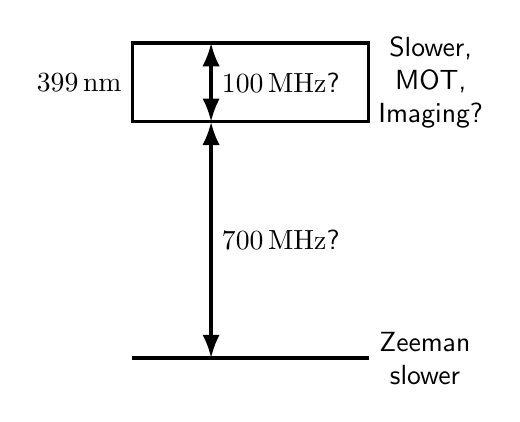
\begin{tikzpicture}
		    		\draw[very thick] (0,0.5) node[left] {\SI{399}{\nano\meter}};
		    		\draw[very thick] (0,1) rectangle ++(3,-1);
		    		\node[right, align=center] at (3,0.5) {Slower,\\ MOT,\\ Imaging?};
		    		\draw[very thick] (0,-3) -- ++(3,0) node[right, align=center] {Zeeman\\slower};
		    		\draw[Latex-Latex, very thick] (1,-3) -- node[midway, right] {\SI{700}{\mega\hertz}?} ++(0,3);
		    		\draw[Latex-Latex, very thick] (1,0) -- node[midway, right] {\SI{100}{\mega\hertz}?} ++(0,1);
		    	\end{tikzpicture}
		    	\caption{Laser frequencies}
		    \end{figure}
		\end{columns}
	\end{frame}
	
	\begin{frame}{Challenges}
		\begin{itemize}
			\item Components selection (fused silica, cubes without glue, ...)
			\item Double-pass AOMs not practical because of strong polarization dependence
			\item Frequency shift for Zeeman slower requires cascade of AOMs
		\end{itemize}
	\end{frame}
	
	\begin{frame}{Discussion}
		\begin{itemize}
			\item Use commercial shutters instead of selfmade shutters?
			\item Separate vertical and horizontal MOT and imaging?
			\item Which laser frequency do we choose?
			\item What are the bandwidth requirements for each of the outputs?
		\end{itemize}
	\end{frame}
	
	%\appendix
\end{document}